\subsection{Red Doméstica}

Para la primera captura, se eligió la red doméstica de uno de los integrantes del grupo. Los dispositivos conectados a la red en este caso fueron, 3 computadoras, 2 teléfonos celulares, un televisor SmartTV y un Apple TV. Todos estos conectados al modem Cisco DPC2420 provisto por el proveedor de internet.
\\
La captura se realizó desde la computadora con dirección IP 192.168.0.30 mediante conexión WIFI y la misma duró aproximadamente 30 minutos.
\\\\
A continuación se pueden observar los diferentes nodos de la red asociados a sus direcciones IP. Los ejes que conectan a un par de nodos representan que entre ellos hubo algún envío de paquetes ARP. El tamaño de cada nodo es proporcional a la cantidad de paquetes que él mismo envió y/o recibió. Esto nos sirve para darnos una idea de la topología de la red.

\begin{figure}[ht!]
  \centering
   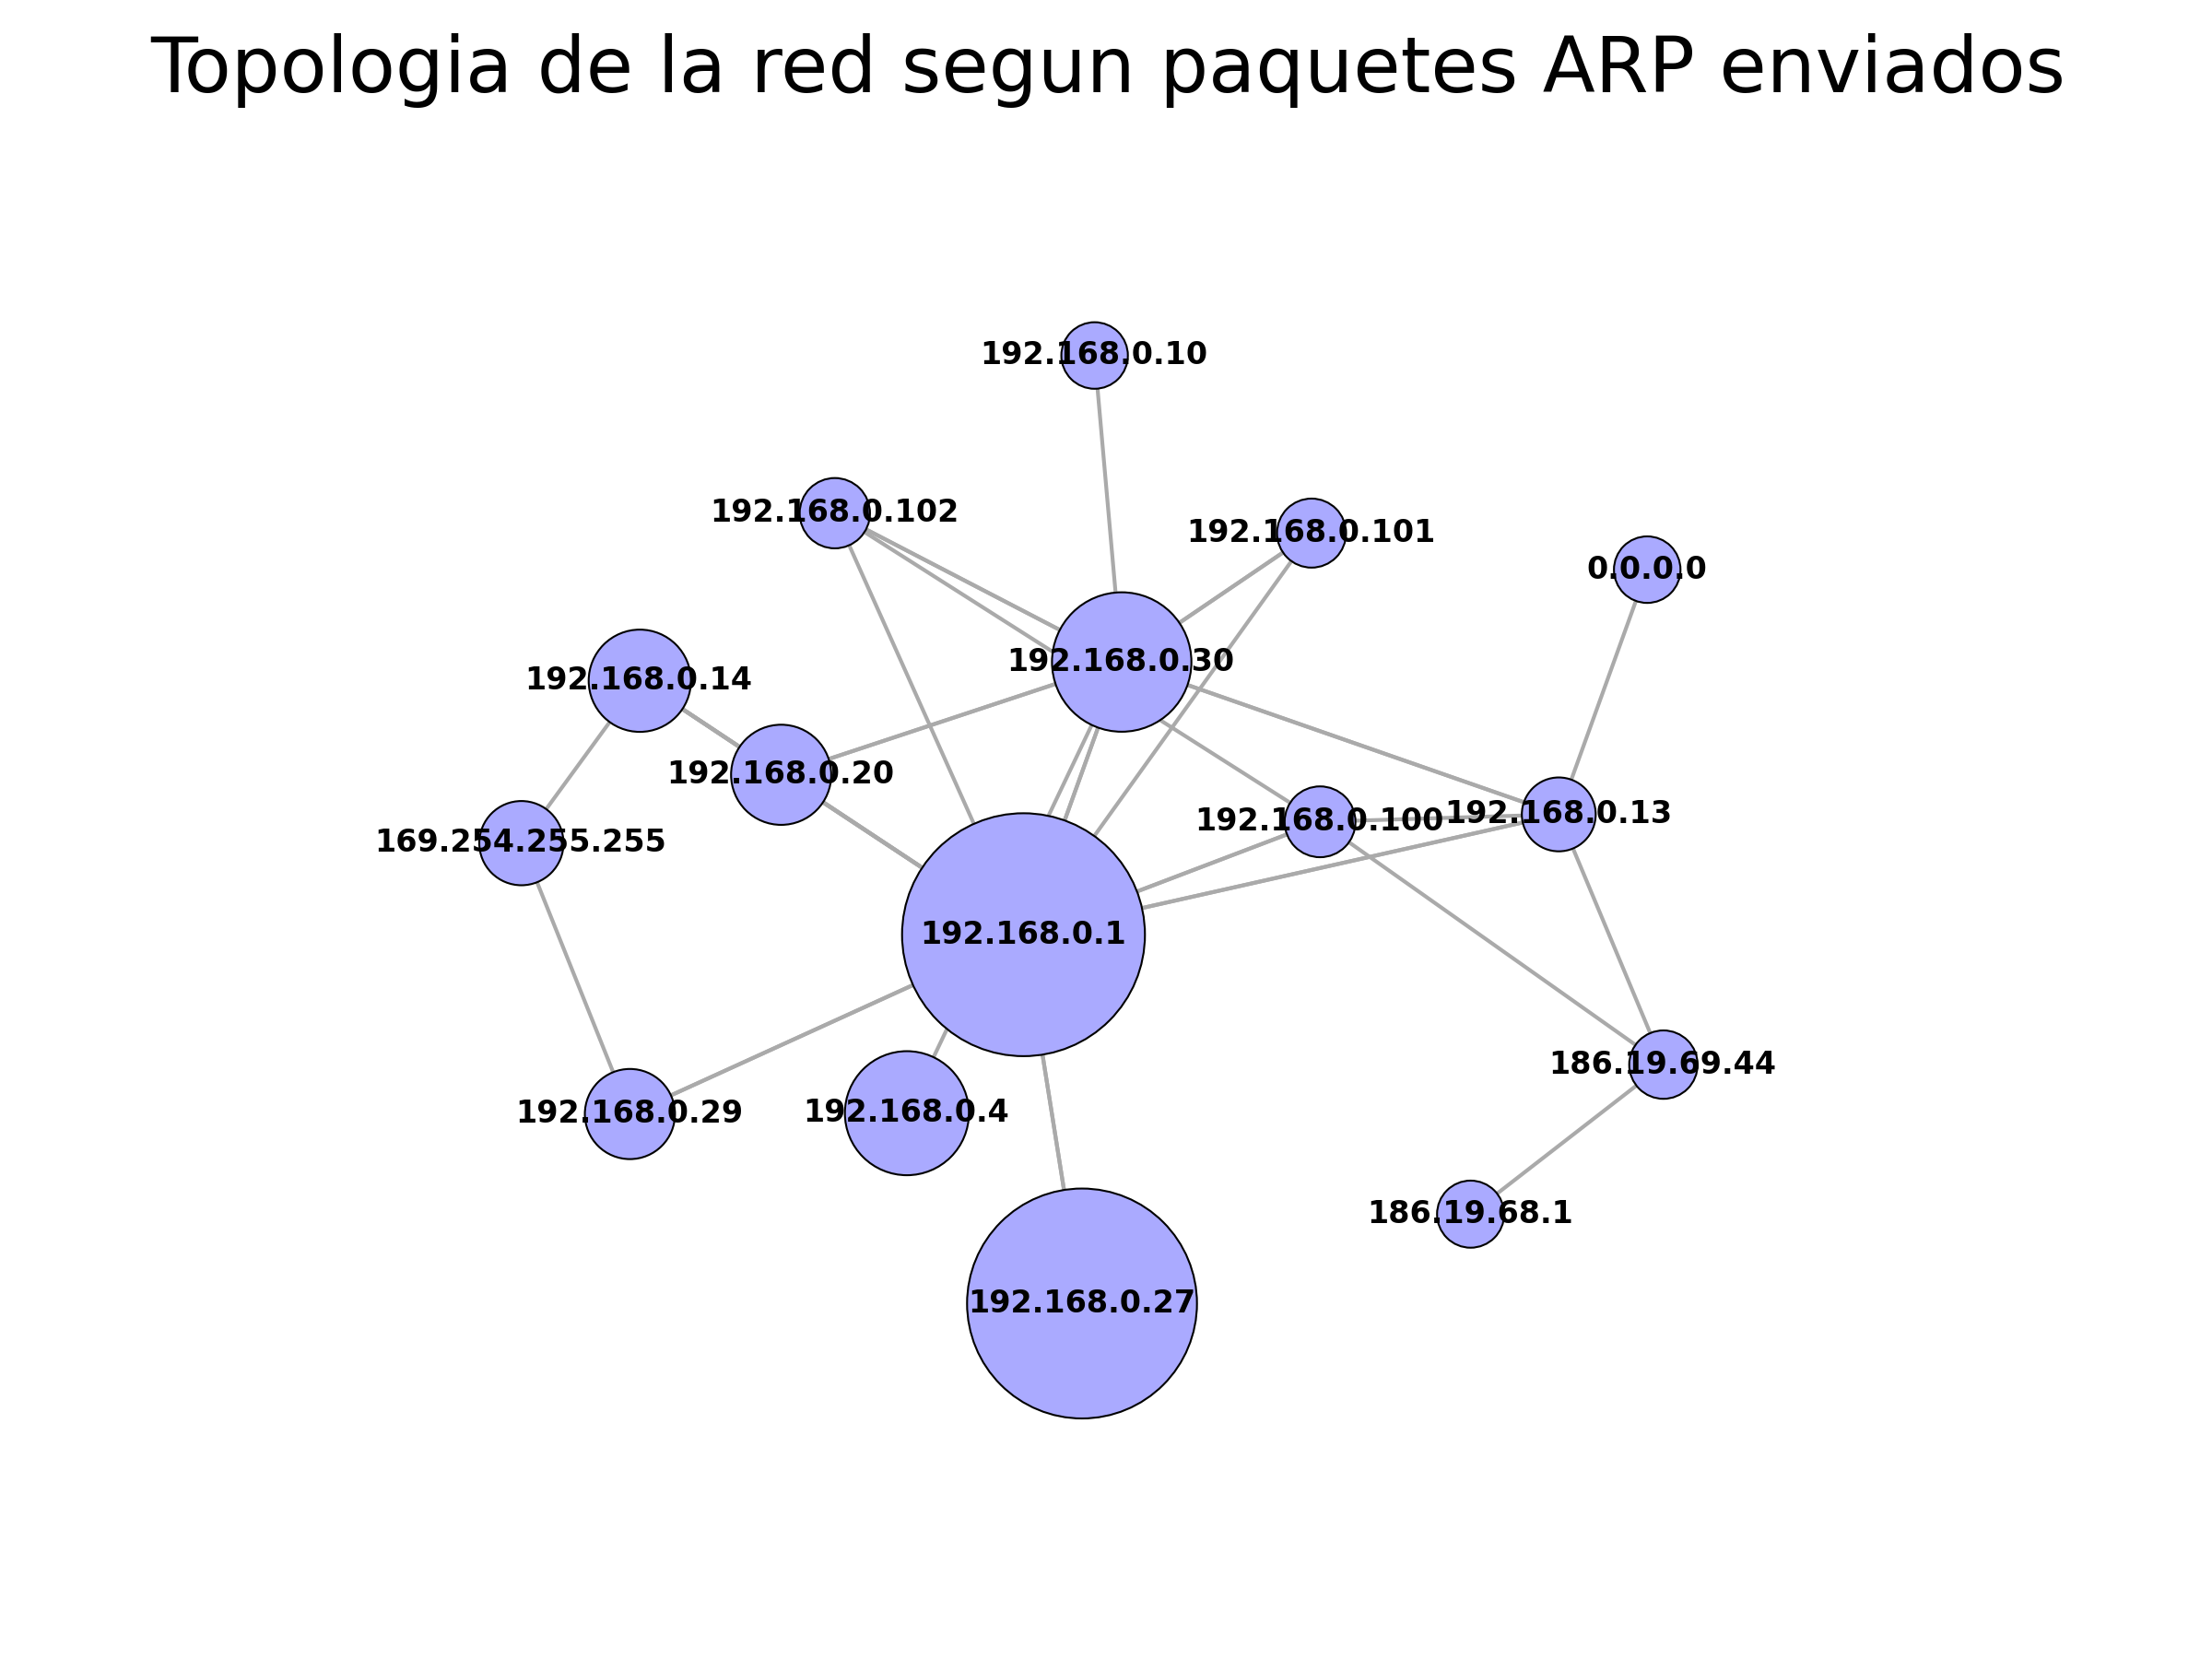
\includegraphics[width=0.7\textwidth]{graficos/domestica_network.png}
  \caption{}
  \label{fig:domestica_network}
\end{figure}

Al ser una red pequeña podemos observar cuáles podrían ser los nodos distinguidos. Uno el que posee la dirección IP 192.168.0.1 que corresponde al modem/router del proveedor de internet. Y el host 192.168.0.27 correspondiente al SmartTV, que según lo que investigamos acerca de su modelo, realiza constantemente búsquedas de nuevos dispositivos conectados a la red.
\\\\
A continuación veremos un gráfico que presenta la cantidad de información de cada nodo en la red. Mediante una recta horizontal se representa el valor de la entropía.

\begin{figure}[ht!]
  \centering
   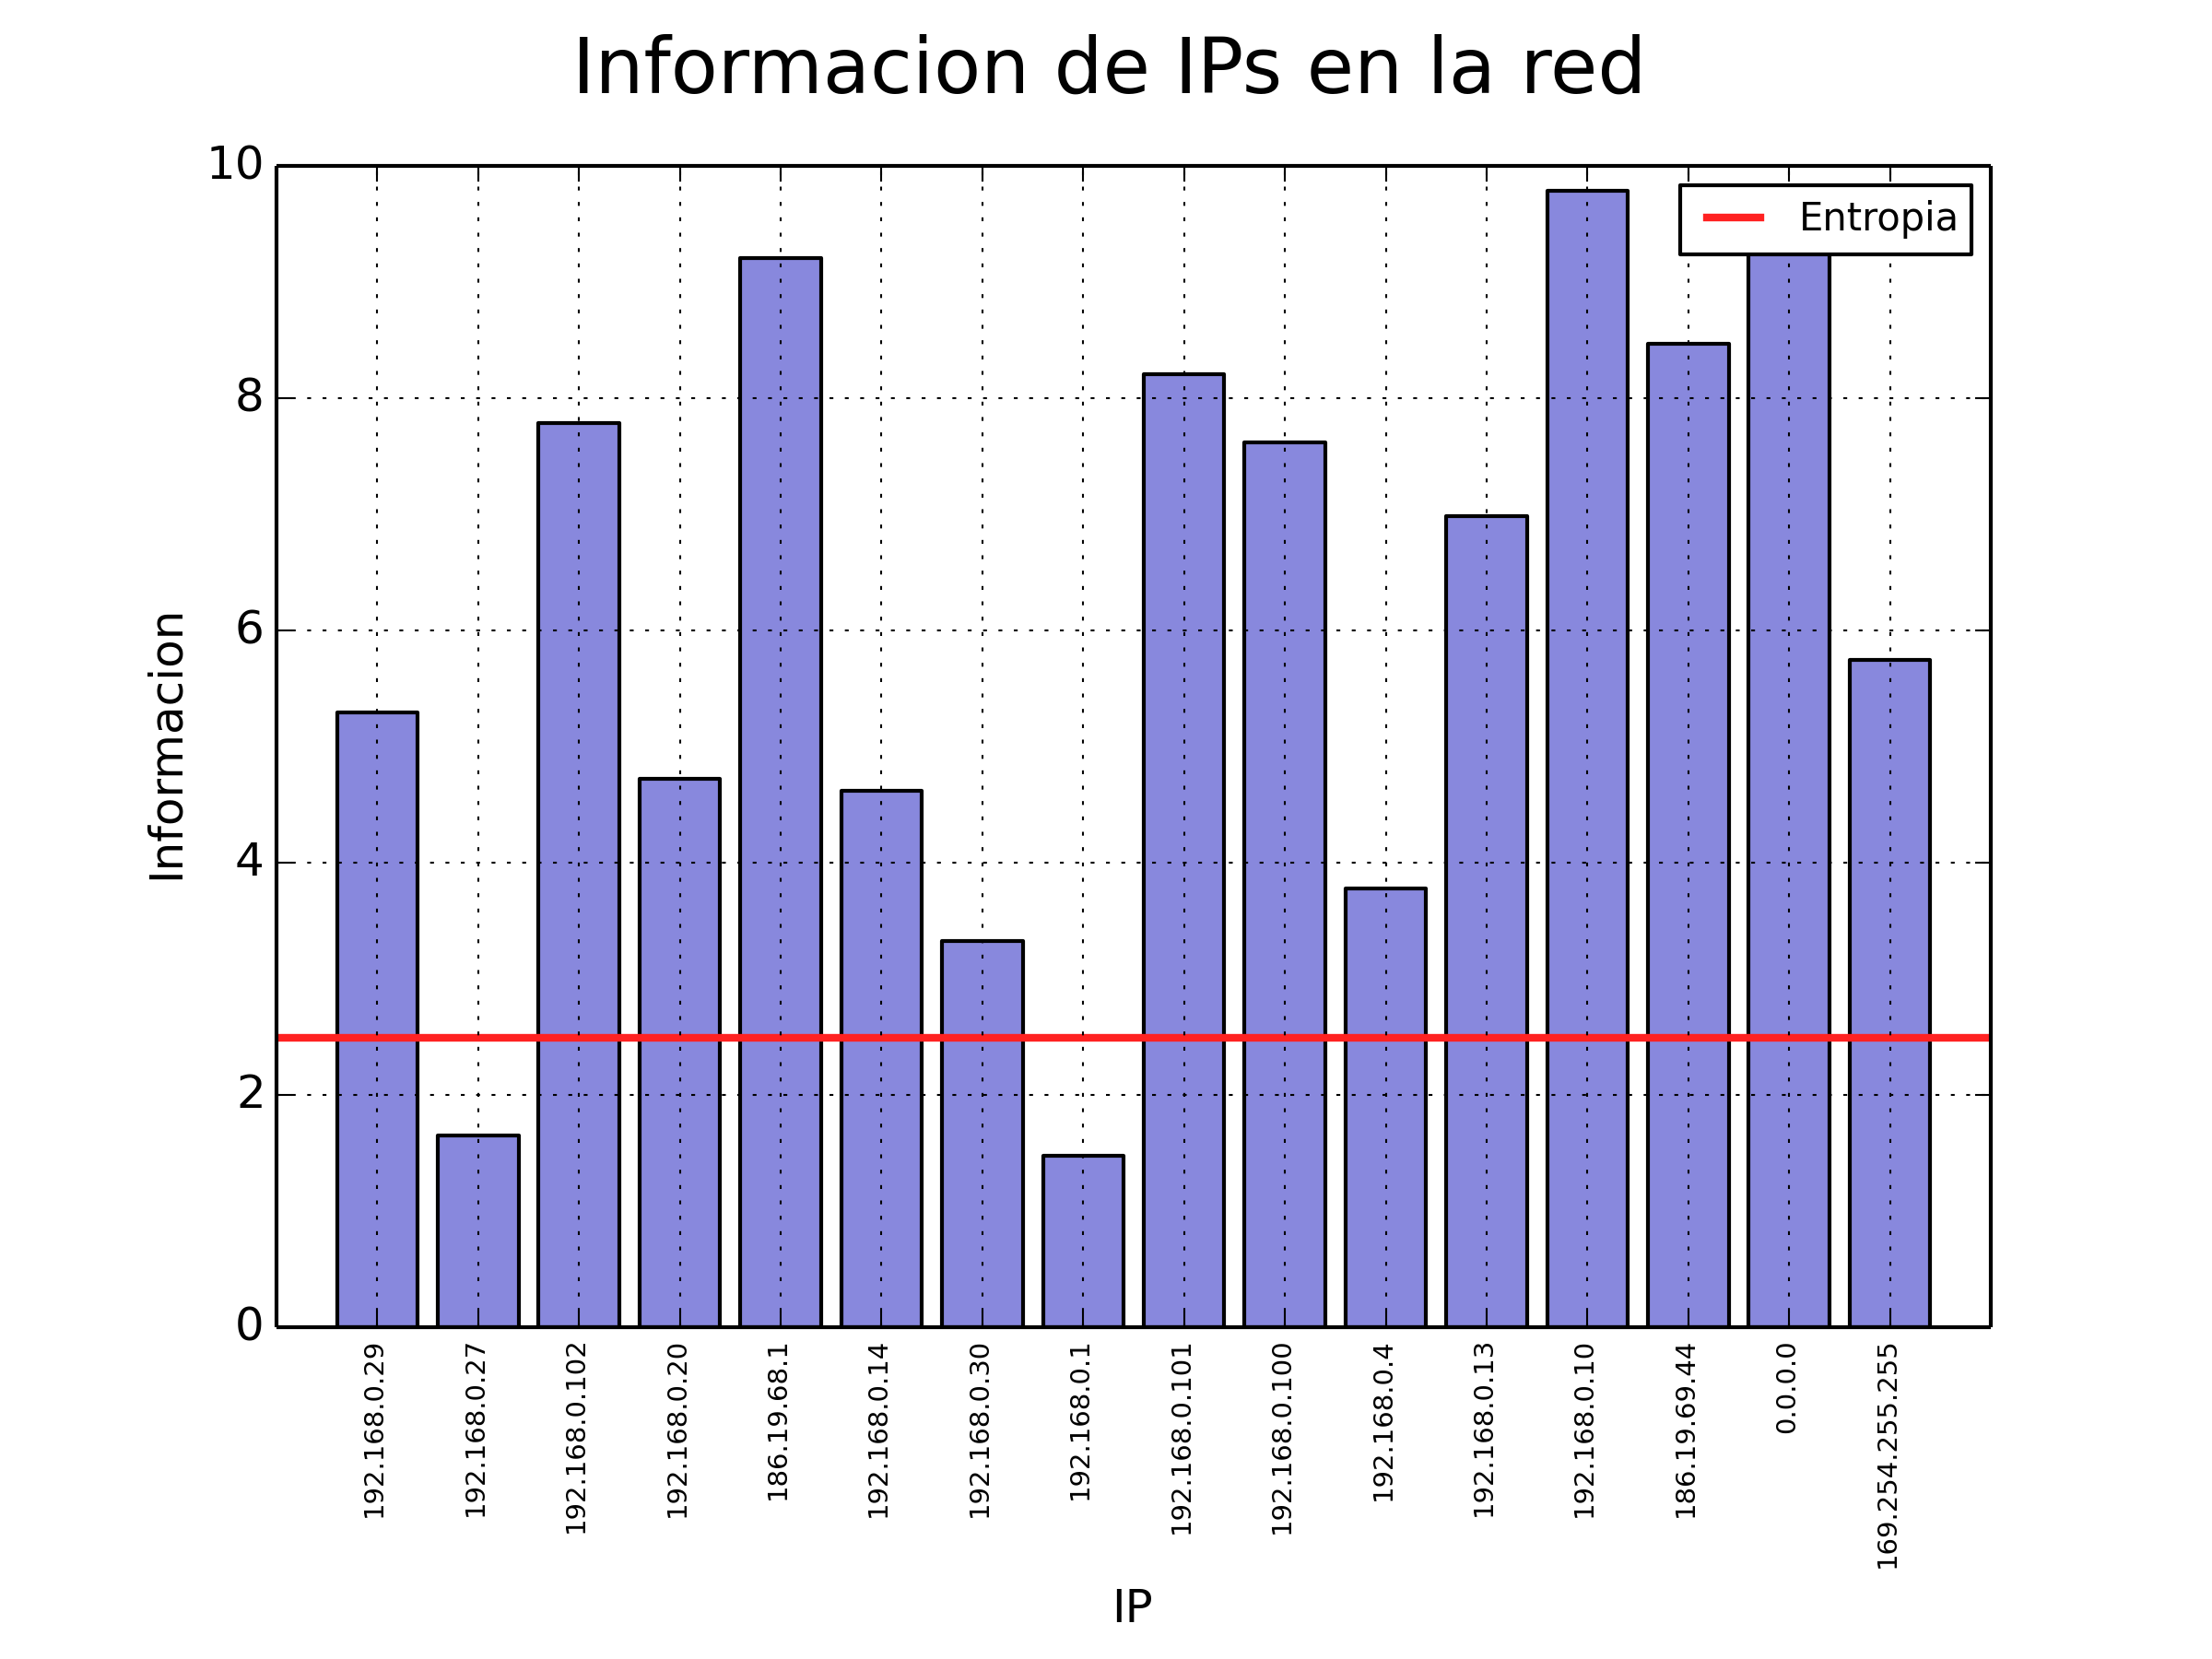
\includegraphics[width=0.7\textwidth]{graficos/domestica_network_information_bars_arp.png}
  \caption{}
  \label{fig:domestica_network_information_bars_arp}
\end{figure}

Podemos observar que los nodos mencionados anteriormente, los que tienen dirección IP 192.168.0.1 y 192.168.0.27, son nodos distinguidos ya que son los únicos para los que su información se encuentra por debajo de la entropía. Es decir que presentaron una alta cantidad de paquetes de tipo ARP en la captura. Por el contrario se pueden ver otros nodos que aportaron mucha información en comparación a la entropía. Este podría ser el caso de algún dispositivo que haya tenido poca participación en el descubrimiento de interfaces mediante el protocolo ARP.
\\\\
A continuación veremos un gráfico mostrando la cantidad de información capturada de cada tipo de protocolo en comparación con el valor de la entropía.

\begin{figure}[ht!]
  \centering
   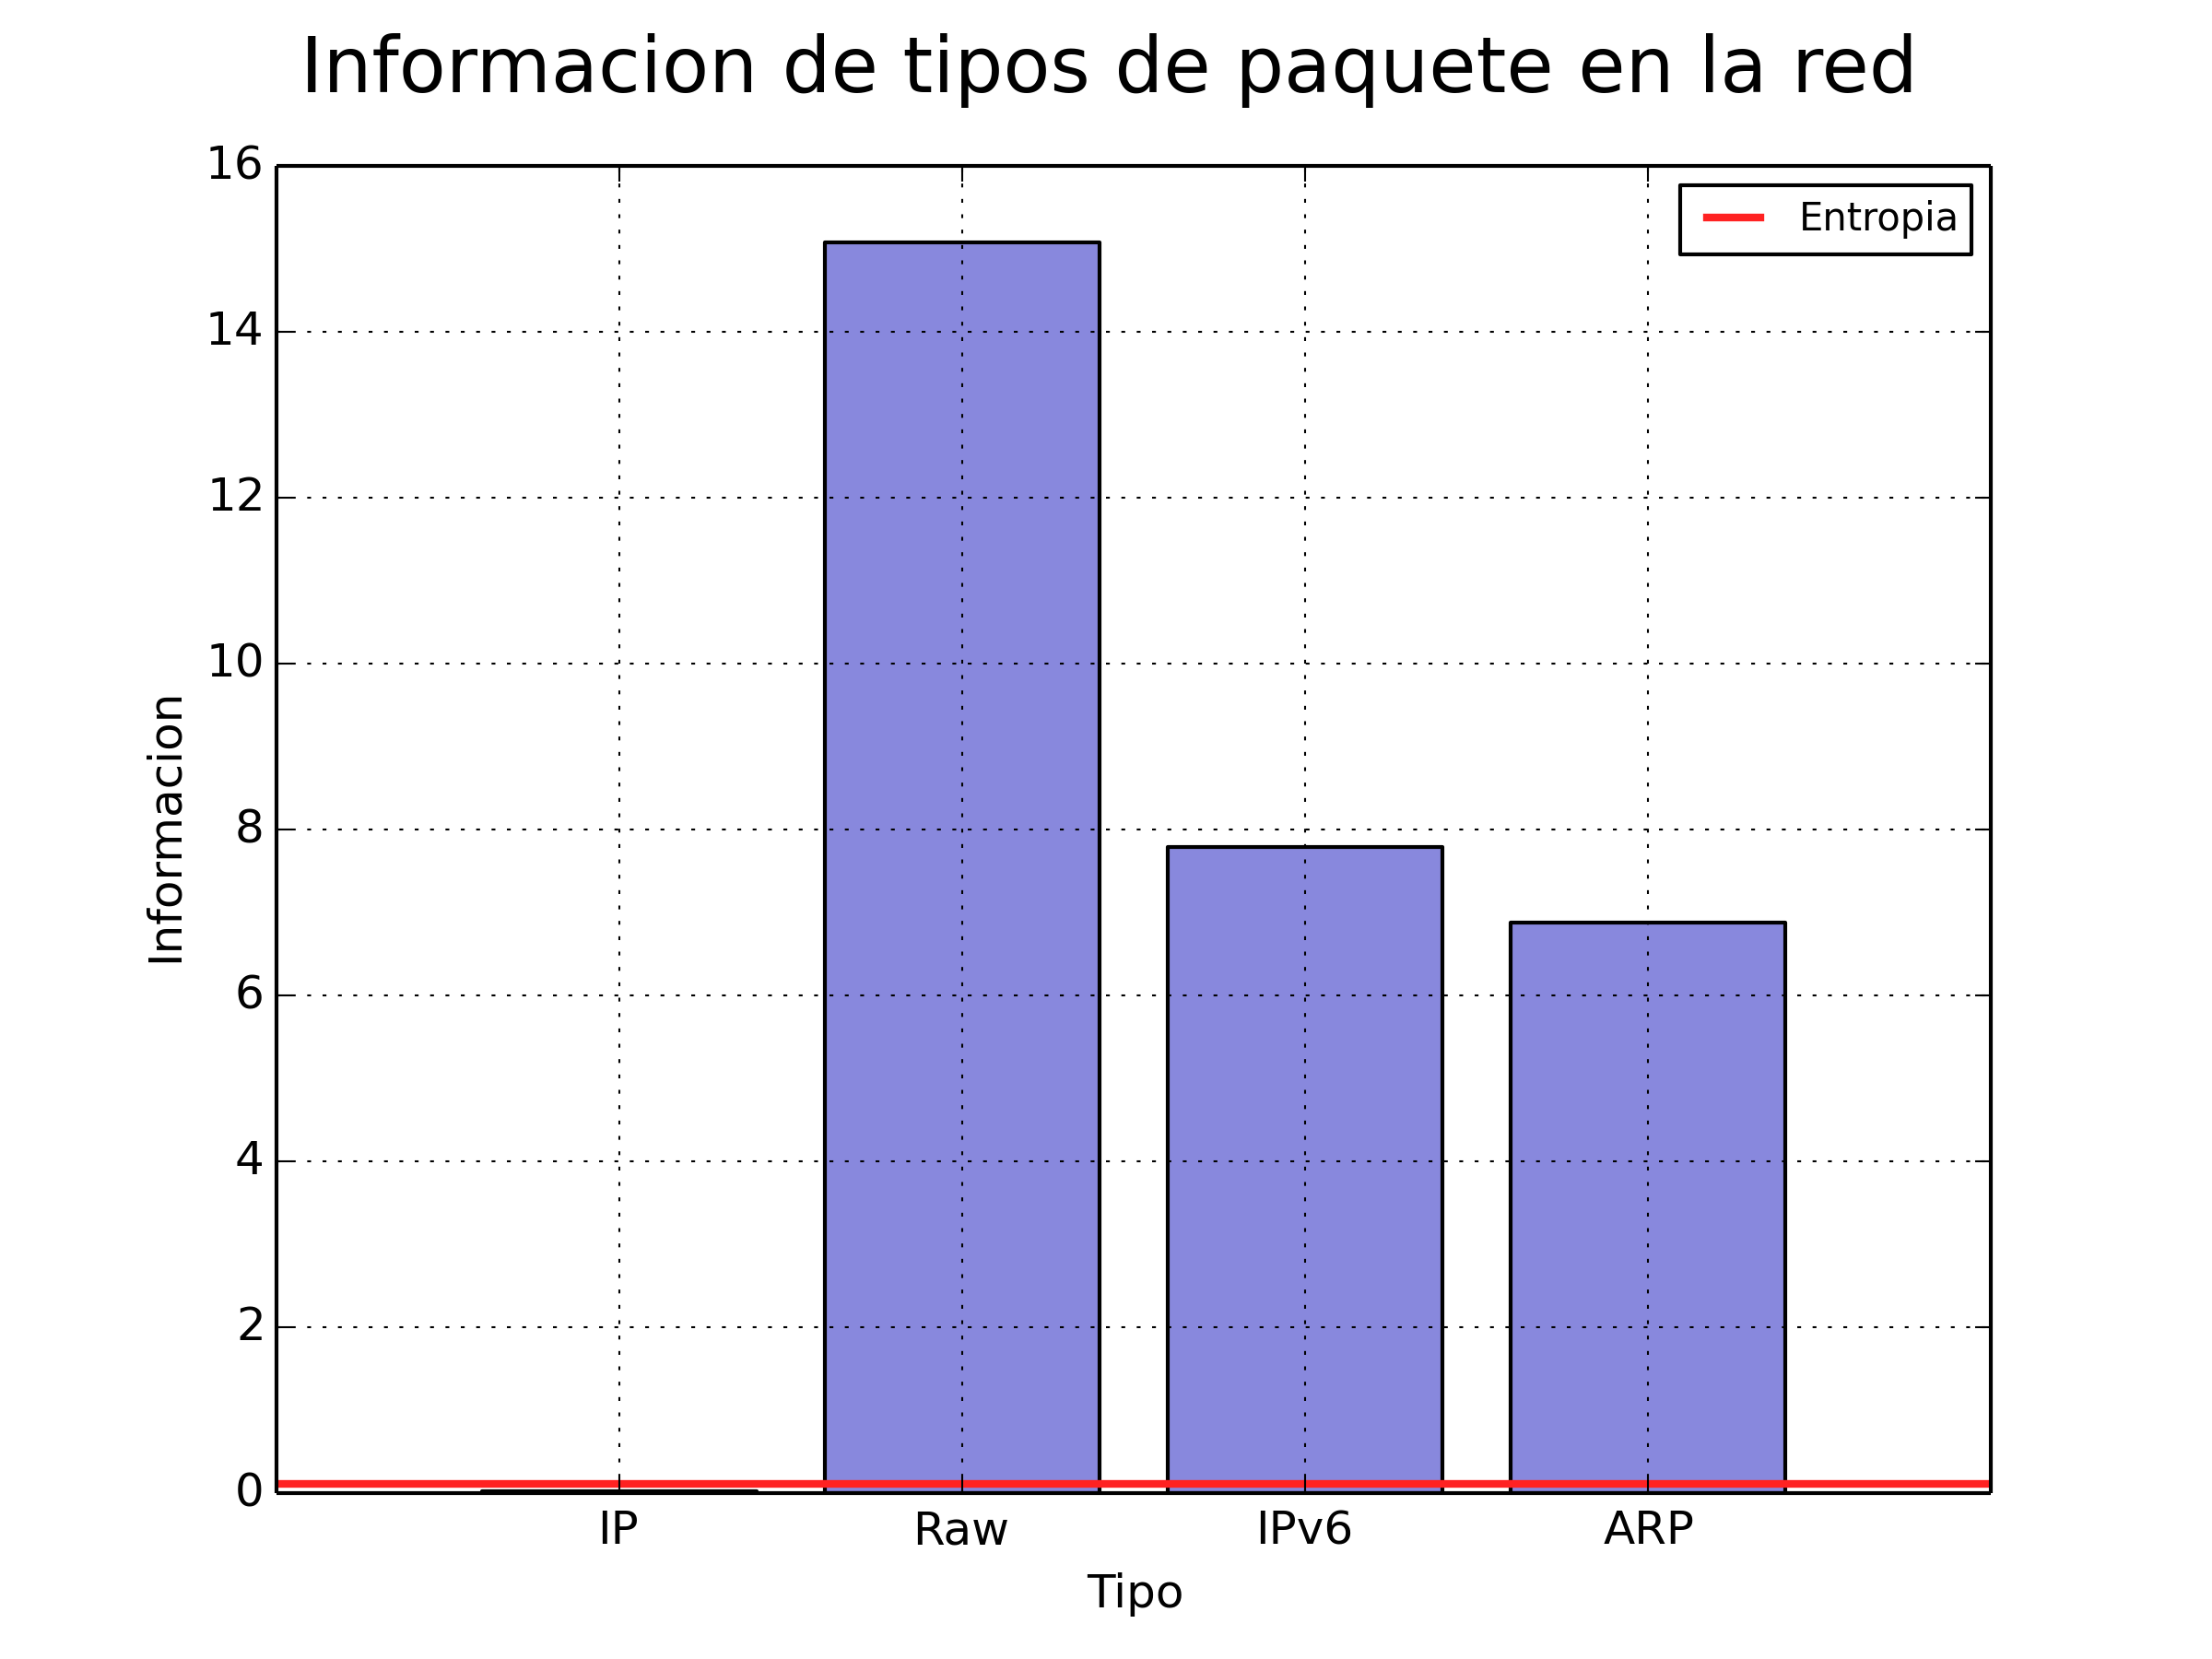
\includegraphics[width=0.7\textwidth]{graficos/domestica_network_information_bars_type.png}
  \caption{}
  \label{fig:domestica_network_information_bars_type}
\end{figure}

Podemos observar que, para este caso, la incidencia de los paquetes ARP en la red es baja en comparación al protocolo IP. Lo mismo ocurre para los protocolos IPv6 y RAW. Es decir que el protocolo IP aporta menor cantidad de información en comparación con los otros tres protocolos. De todas formas, El protocolo ARP tuvo mayor frecuencia, y aportó menor información, que los protocolos IPv6 y RAW. Esto puede darse dado que estos últimos tienen menor uso que ARP.